%\documentclass[notes=show,xcolor=table]{beamer}
\documentclass[xcolor=table]{beamer}
% german and utf8
\usepackage[ngerman]{babel}
\usepackage[utf8]{inputenc}

\usepackage{lmodern}
% Das Paket lmodern erspart die folgenden Warnungen:
% LaTeX Font Warning: Font shape `OT1/cmss/m/n' in size <4> not available
% (Font)              size <5> substituted on input line 22.
% LaTeX Font Warning: Size substitutions with differences
% (Font)              up to 1.0pt have occurred.

% beamer style
%\usepackage{beamerthemeshadow}
\usetheme{Warsaw}
\usecolortheme[named=blue]{structure}


\setbeamertemplate{footline}{
	\leavevmode%
	\hbox{%
		\begin{beamercolorbox}[wd=.15\paperwidth,ht=2.25ex,dp=1ex,center]{date in head/foot}%
			\usebeamerfont{date in head/foot}\insertshortdate{}
		\end{beamercolorbox}%
%		\begin{beamercolorbox}[wd=.2\paperwidth,ht=2.25ex,dp=1ex,center]{author in head/foot}%
%			\usebeamerfont{author in head/foot}\insertshortauthor%~~(\insertshortinstitute)
%		\end{beamercolorbox}%
		\begin{beamercolorbox}[wd=.7\paperwidth,ht=2.25ex,dp=1ex,center]{title in head/foot}%
			\usebeamerfont{title in head/foot}\insertshorttitle
		\end{beamercolorbox}%
		\begin{beamercolorbox}[wd=.15\paperwidth,ht=2.25ex,dp=1ex,right]{date in head/foot}%
			\usebeamerfont{date in head/foot}\insertframenumber{} / \inserttotalframenumber{}
		\end{beamercolorbox}%
	}%
	\vskip0pt%
}

% allow colored tables
% http://tex.stackexchange.com/questions/68371/how-to-highlight-table-rows-by-colors-in-beamer
% for a more sophisticated solution see http://tex.stackexchange.com/a/18430/10327
\rowcolors{1}{gray!30}{gray!10}

\makeatletter
\def\rowcolor{\noalign{\ifnum0=`}\fi\bmr@rowcolor}
\newcommand<>{\bmr@rowcolor}{%
	\alt#1%
		{\global\let\CT@do@color\CT@@do@color\@ifnextchar[\CT@rowa\CT@rowb}%
		{\ifnum0=`{\fi}\@gooble@rowcolor}%
}

\newcommand{\@gooble@rowcolor}[2][]{\@gooble@rowcolor@}
\newcommand{\@gooble@rowcolor@}[1][]{\@gooble@rowcolor@@}
\newcommand{\@gooble@rowcolor@@}[1][]{\ignorespaces}
\makeatother

\usepackage{color, colortbl}
\definecolor{LRed}{rgb}{1,.8,.8}
\definecolor{MRed}{rgb}{1,.6,.6}
\definecolor{HRed}{rgb}{1,.2,.2}

% speech bubbles
% http://tex.stackexchange.com/questions/38805/simple-speech-bubbles-arrows-or-balloon-like-shapes-in-beamer
\usepackage{tikz}
\usetikzlibrary{calc,shapes.callouts,shapes.arrows}
% usage: \arrowthis{There is}{Corot}
\newcommand{\arrowthis}[2]{
	\tikz[remember picture,baseline]{\node[anchor=base,inner sep=0,outer sep=0]%
		(#1) {\underline{#1}};
		\node[overlay,single arrow,draw=none,fill=red!50,anchor=tip,rotate=60] 
	at (#1.south) {#2};}%
}%
\newcommand{\speechthis}[2]{
	\tikz[remember picture,baseline]{\node[anchor=base,inner sep=0,outer sep=0]%
		(#1) {\underline{#1}};\node[overlay,ellipse callout,fill=blue!50] 
	at ($(#1.north)+(-.5cm,0.8cm)$) {#2};}%
}%
\newcommand{\bubblethis}[2]{
	\tikz[remember picture,baseline]{\node[anchor=base,inner sep=0,outer sep=0]%
		(#1) {\underline{#1}};\node[overlay,cloud callout,callout relative pointer={(0.2cm,-0.7cm)},%
	aspect=2.5,fill=yellow!90] at ($(#1.north)+(-0.5cm,1.6cm)$) {#2};}%
}%
\newcommand{\pointthis}[2]{
	\tikz[remember picture,baseline]{\node[anchor=base,inner sep=0,outer sep=0]%
		(#1) {\underline{#1}};\node[overlay,rectangle callout,%
	callout relative pointer={(0.2cm,0.7cm)},fill=green!50] at ($(#1.north)+(-.5cm,-1.4cm)$) {#2};}%
}%


% allow strikethrough with \sout
% http://tex.stackexchange.com/questions/23711/strikethrough-text
%\usepackage{ulem}

% multimedia
% http://mo.mathematik.uni-stuttgart.de/inhalt/aussage/aussage1325/
% http://tex.stackexchange.com/questions/429/animation-in-pdf-presentations-without-adobe-reader
% http://www.ctan.org/pkg/animate

% againframe 
% http://stackoverflow.com/questions/171708/latex-beamer-package-change-frame-title-in-againframe
% http://tex.stackexchange.com/questions/31031/beamer-repeat-variations-of-a-frame

% todo notes
% http://tex.stackexchange.com/questions/11177/how-to-write-hidden-notes-in-a-latex-file

% http://www.texample.net/tikz/examples/feature/overlays/
% http://tex.stackexchange.com/questions/14769/add-more-anchors-to-standard-tikz-nodes

%\beamersetuncovermixins{\opaqueness<1>{25}}{\opaqueness<2->{15}}
% sorgt dafuer das die Elemente die erst noch (zukuenftig) kommen nur schwach angedeutet erscheinen
% klappt auch bei Tabellen, wenn teTeX verwendet wird\ldots

% http://tex.stackexchange.com/questions/16357/how-can-i-position-an-image-in-an-arbitrary-position-in-beamer
\usepackage{tikz}
%\usetikzlibrary{calc, trees, positioning, arrows, shapes, shapes.multipart, shadows, matrix, decorations.pathreplacing, decorations.pathmorphing}
\usetikzlibrary{arrows}%, shapes}%, shapes.multipart}%, automata}
\tikzset{
  every boverlay node/.style={
    draw=black,fill=white,rounded corners,anchor=north west,
  },
}
\tikzset{
  every toverlay node/.style={
	anchor=center
  },
}
\tikzset{
  every overlay node/.style={
    draw=white,fill=white,rounded corners,anchor=north west,
  },
}
% Usage:
% \tikzoverlay at (-1cm,-5cm) {content};%
% or
% \tikzoverlay[text width=5cm] at (-1cm,-5cm) {content};%
\def\tikzboverlay{% A bordered overlay
   \tikz[baseline,overlay]\node[every boverlay node]
}%
\def\tikztoverlay{% A transparent overlay
   \tikz[baseline,overlay]\node[every toverlay node]
}%
\def\tikzoverlay{% A non-transparent unbordered overlay
   \tikz[baseline,overlay]\node[every overlay node]
}%



\title{Optimierung von Sensornetzen}
\author{Daniel Kniese\and\\Mitja Richter}
\date{1. März 2013}

\begin{document}

	\begin{frame}
		\titlepage
	\end{frame}

	\begin{frame}
		\frametitle{Inhaltsverzeichnis}
		\tableofcontents
	\end{frame}


	\AtBeginSection[]{
		\begin{frame}
			\frametitle{Inhaltsverzeichnis}
			\tableofcontents[currentsection]
		\end{frame}
	}
	
	\section{Sensornetze}
	\subsection{statische Netze}
		\begin{frame}
			\frametitle{Anwendungen statischer Netze}
			\tikztoverlay at (5.35cm,-0.44cm) (atom) {
			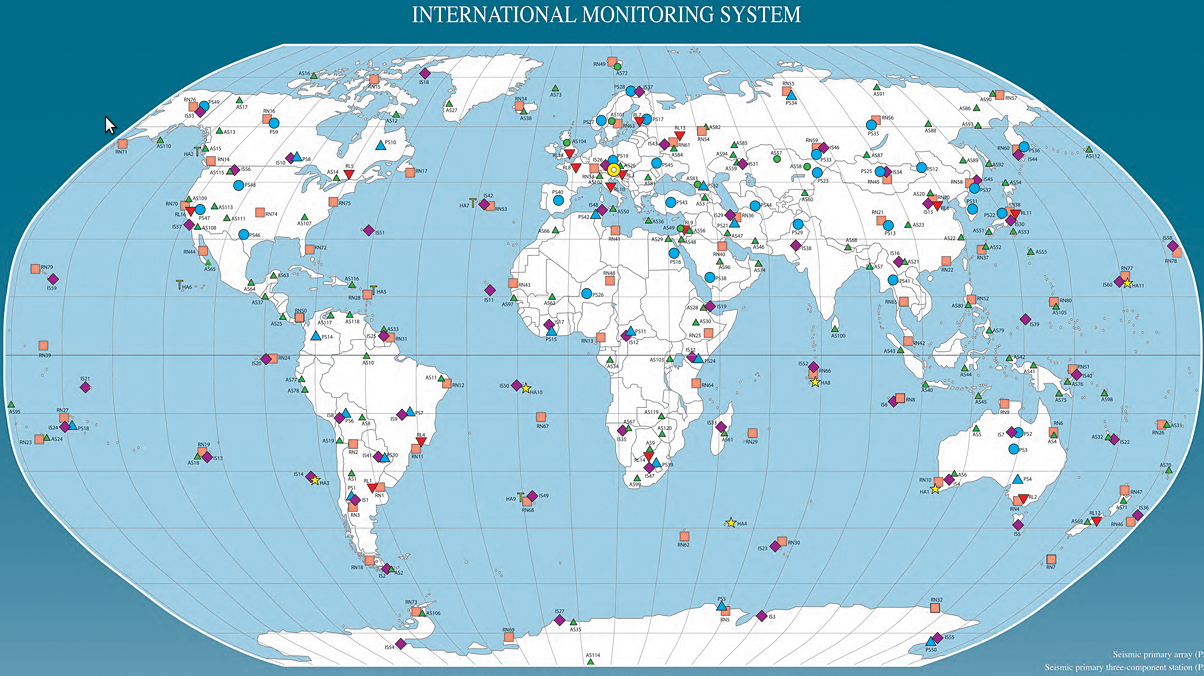
\includegraphics[scale=0.3]{bilder/atomwaffen.png}
		};%
		\note{Organisation des Vertrags über das umfassende Verbot von Nuklearversuchen(CTBTO) 50 primäre und 120 sekundäre seismologische Messstationen, die seismische Aktivitäten aufzeichnet und versucht nukleare Explosionen von Erdbeben zu unterscheiden}
		\end{frame}
		\begin{frame}
			\frametitle{Vorteile statischer Sensornetze}
		\end{frame}
		
	\subsection{mobile Netze}
		\begin{frame}
			\frametitle{Anwendungen mobiler Sensornetze}
			\begin{itemize}
				\item militärische Überwachung (Beispiele)
				\item Überwachung des Ökosystems (Beispiele)
			\end{itemize}
		\end{frame}
		\begin{frame}
			\frametitle{Vorteile mobiler Netze}
			
		\end{frame}
	\section{Problemaufbau}
	\subsection{Einsatzgebiet}
		\begin{frame}
			\frametitle{Einsatzgebiet}
			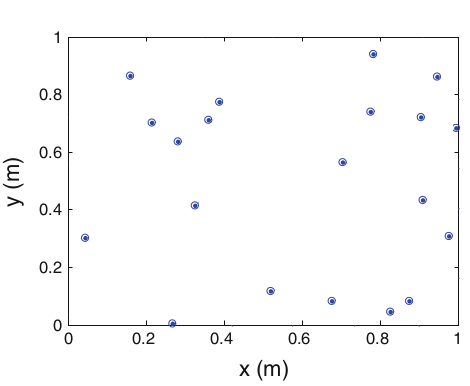
\includegraphics[scale=0.48]{bilder/aufbau1.png}
			\note{wir haben eine beliebige Anzahl von Robotern mit entsprechenden Sensoren ausgestattet. diese werden jetzt zufällig in einer abgeschlossenen konvexen Umgebung eingesetzt.}
		\end{frame}
	\subsection{Sensorfunktion}
		\begin{frame}
			\frametitle{Sensorfunktion}
			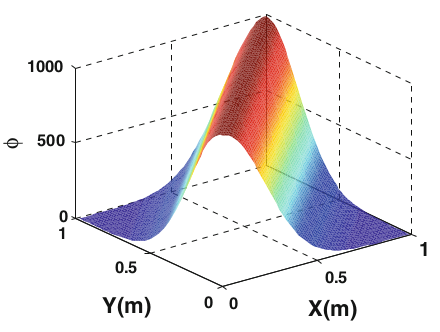
\includegraphics[scale=0.48]{bilder/sensor1.png}
			\tikzoverlay at (-0.4cm,5cm) {\small $\phi(x,y)=a\cdot exp(-b(x-y)^2)$};
			\tikzoverlay at (-0.4cm,4.5cm) {\small mit $a=1000$ und $b=-10$};
		\note{keine Linearkombination von Standardnormalverteilungen}
		\end{frame}
		\begin{frame}
			\frametitle{Sensorfunktion}
			\tikztoverlay at (2.35cm,-0.44cm) (aufbau) {
			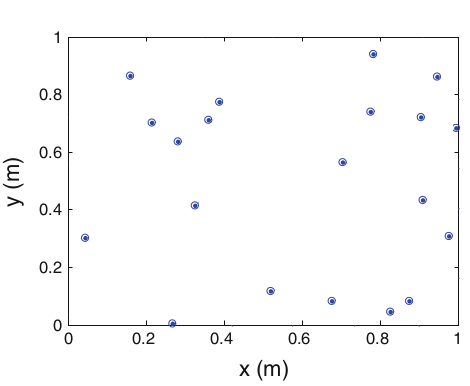
\includegraphics[scale=0.35]{bilder/aufbau1.png}};
			\tikztoverlay at (8cm,-0.44cm) (sensor) {
			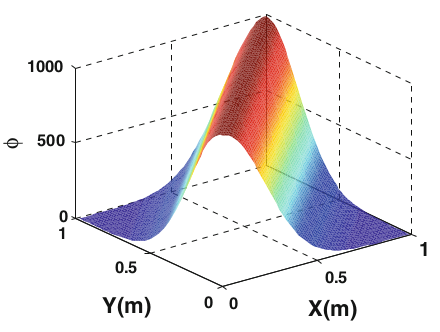
\includegraphics[scale=0.35]{bilder/sensor1.png}};
		\end{frame}
		
		\begin{frame}
			\frametitle{Aufteilung}
			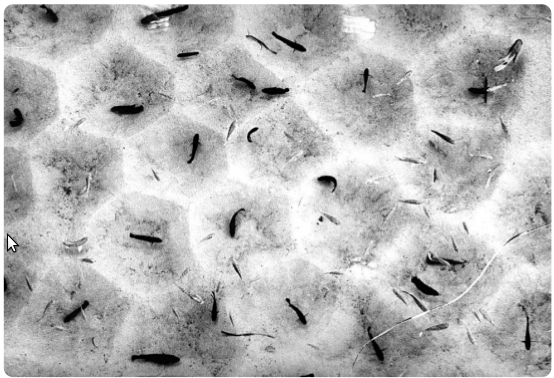
\includegraphics[scale=0.5]{bilder/vonoroiFische.png}
			\note{Es gibt eine afrikanische Buntbarschart, die ihr territoriales Verhalten ausüben, indem sie untereinander das Gebiet in sich nicht überschneidende Teilgebiete unterteilen. Sie bilden kleine Gruben deren Ränder dann ein Polygonmuster bilden. Mann kennt dieses Muster auch unter dem Namen Vonoroipartitionen.}
		\end{frame}
		\subsection{Vonoroi-Partitionen}
		\begin{frame}
			\frametitle{Vonoroi-Partitionen}
			Gegeben sei:
			\begin{itemize}
				\item[•] Menge $S\subset \mathbb{R}^2$
				\item[•] Menge $P=\{p_1,p_2,...,p_n\} \subset S$
			\end{itemize}
			Dann sei die Menge der Vonoroi-Partitionen $\{V_1(P),V_2(P),...,V_n(p)\}$ gegeben durch:
			\begin{itemize}
				\item[•] $V_i(P)=\{q \in S| \|q-p_i\|\leq \|q-p_j \|, \forall p_j \in P\}$
			\end{itemize}
		\end{frame}
		\begin{frame}
			\frametitle{Vonoroi-Partitionen}
			\tikztoverlay at (5.35cm,-0.44cm) (atom) {
			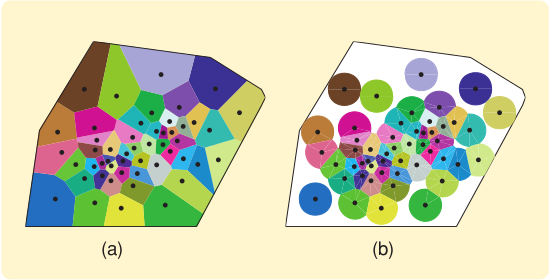
\includegraphics[scale=0.6]{bilder/vonoroi.png}
		};%
		\end{frame}
		\begin{frame}
			\frametitle{Vonoroi-Partitionen}
			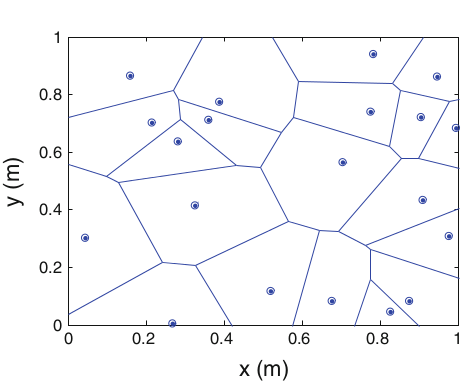
\includegraphics[scale=0.48]{bilder/aufbau2.png}
		\end{frame}
		\subsection{Sensorfunktion}
		\begin{frame}
			\frametitle{Vonoroi-Partitionen}
			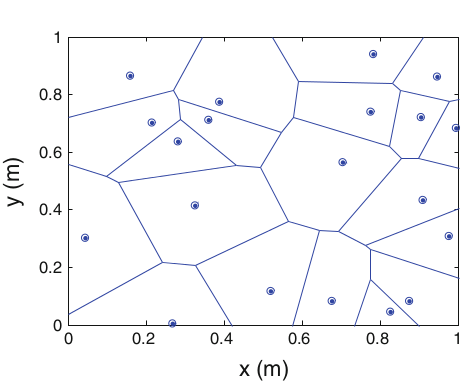
\includegraphics[scale=0.48]{bilder/aufbau2.png}
		\end{frame}
	\subsection{allgemein}
	\subsection{ohne Sensorfunktion}
	\section{Wofür wird KI gebraucht}
	\section{Ergebnisse}
	\section{Fazit}
\end{document}
